\documentclass{article}
\usepackage{fullpage}
\usepackage[utf8]{inputenc}
\usepackage[T1, T2A]{fontenc}
\usepackage[english, russian]{babel}
\usepackage{indentfirst}
\usepackage{graphicx}
\selectlanguage{russian}
\graphicspath{{./graphics/}}

\begin{document}
\begin{titlepage}
    \begin{center}
        \normalsize
        МГТУ им Н.Э. Баумана, кафедра ИУ5 \\
        \vspace*{1cm}
        \LARGE
        \textbf{Лабораторная работа №3 по дисцилине "РИП"}

        \vspace{0.5cm}
    \end{center}
    \vfill

    \begin{flushright}
        \textbf{Выполнил:} Никольский Даниил, ИУ5-51б \\
        \textbf{Проверил:} Гапанюк Юрий Евгеньевич, ИУ5 \\
    \end{flushright}
    \vspace{1.5cm}
    \begin{flushleft}
        \textbf{Дата: \today} \\
        \textbf{Подпись: Никольский Д.Р.} \\
    \end{flushleft}
\end{titlepage}

\tableofcontents
\newpage

\section{Задание}
\begin{enumerate}
    \item Программа должна быть разработана в виде консольного приложения на языке Python 3.

    \item Все файлы проекта (кроме основного файла main.py) должны располагаться в пакете lab\_python\_oop.

    \item Абстрактный класс «Геометрическая фигура» содержит абстрактный метод для вычисления площади фигуры.

    \item Класс «Цвет фигуры» содержит свойство для описания цвета геометрической фигуры.

    \item Класс «Прямоугольник» наследуется от класса «Геометрическая фигура». Класс должен содержать конструктор по параметрам «ширина», «высота» и «цвет». В конструкторе создается объект класса «Цвет фигуры» для хранения цвета. Класс должен переопределять метод, вычисляющий площадь фигуры.

    \item Класс «Круг» создается аналогично классу «Прямоугольник», задается параметр «радиус».

    \item Класс «Квадрат» наследуется от класса «Прямоугольник». Класс должен содержать конструктор по длине стороны.

    \item Для классов «Прямоугольник», «Квадрат», «Круг»:

    \item Определите метод repr, который возвращает в виде строки основные параметры фигуры, ее цвет и площадь.

    \item Название фигуры («Прямоугольник», «Квадрат», «Круг») должно задаваться в виде поля данных класса и возвращаться методом класса.

    \item В корневом каталоге проекта создайте файл main.py для тестирования Ваших классов. Создайте следующие объекты и выведите о них информацию в консоль:
          \begin{enumerate}
              \item Прямоугольник синего цвета шириной 3 и высотой 2.

              \item Круг зеленого цвета радиусом 5.

              \item Квадрат красного цвета со стороной 5.
          \end{enumerate}
\end{enumerate}

\section{Исходный код}
\subsection{color.py}
\begin{verbatim}
class Color:
def __init__(self):
    self._color = None

def get_color(self):
    return self._color

def set_color(self, color):
    self._color = color

def del_color(self):
    del self._color

color = property(get_color, set_color, del_color, "Color property")
\end{verbatim}
\subsection{figure.py}
\begin{verbatim}
    from abc import ABC, abstractmethod
from math import pi

from lab3.lab_python_oop.color import Color


class Figure(ABC):
    @abstractmethod
    def area(self):
        pass


class Rectangle(Figure):
    def __init__(self, height, width, color):
        self.height = height
        self.width = width

        self.color = Color()
        self.color.set_color(color)

        self.figure_name = "Rectangle"

    def area(self):
        return self.width * self.height

    def __repr__(self):
        return f'<{self.figure_name}, \
                 w: {self.width}, \
                 h: {self.height}, \
                 c: {self.color.get_color()}, \
                 a: {self.area()}>'


class Circle(Figure):
    def __init__(self, rad, color):
        self.rad = rad

        self.color = Color()
        self.color.set_color(color)

        self.figure_name = "Circle"

    def area(self):
        return pi * self.rad ** 2

    def __repr__(self):
        return f'<{self.figure_name}, \
                r: {self.rad}, \
                c: {self.color.get_color()}, \
                a: {self.area()}>'


class Square(Rectangle):
    def __init__(self, a, color):
        super().__init__(a, a, color)

        self.figure_name = "Square"

    def __repr__(self):
        return f'<{self.figure_name}, \
                s: {self.width}, \
                c: {self.color.get_color()}, \
                a: {self.area()}>'

\end{verbatim}
\subsection{main.py}
\begin{verbatim}
from lab3.lab_python_oop.figure import Rectangle, Circle, Square


def main():
    rect = Rectangle(2, 3, 'blue')
    circle = Circle(5, 'green')
    square = Square(5, 'red')
    print(rect)
    print(circle)
    print(square)


if __name__ == '__main__':
    main()

\end{verbatim}
\newpage
\section{Результат}
\begin{figure}[!h]
    \centering
    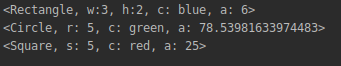
\includegraphics{result.png}
    \caption{}
    \label{}
\end{figure}
    

\end{document}